\documentclass[journal, a4paper]{IEEEtran}

% some very useful LaTeX packages include:

%\usepackage{cite}      % Written by Donald Arseneau
                        % V1.6 and later of IEEEtran pre-defines the format
                        % of the cite.sty package \cite{} output to follow
                        % that of IEEE. Loading the cite package will
                        % result in citation numbers being automatically
                        % sorted and properly "ranged". i.e.,
                        % [1], [9], [2], [7], [5], [6]
                        % (without using cite.sty)
                        % will become:
                        % [1], [2], [5]--[7], [9] (using cite.sty)
                        % cite.sty's \cite will automatically add leading
                        % space, if needed. Use cite.sty's noadjust option
                        % (cite.sty V3.8 and later) if you want to turn this
                        % off. cite.sty is already installed on most LaTeX
                        % systems. The latest version can be obtained at:
                        % http://www.ctan.org/tex-archive/macros/latex/contrib/supported/cite/

\usepackage{graphicx}   % Written by David Carlisle and Sebastian Rahtz
                        % Required if you want graphics, photos, etc.
                        % graphicx.sty is already installed on most LaTeX
                        % systems. The latest version and documentation can
                        % be obtained at:
                        % http://www.ctan.org/tex-archive/macros/latex/required/graphics/
                        % Another good source of documentation is "Using
                        % Imported Graphics in LaTeX2e" by Keith Reckdahl
                        % which can be found as esplatex.ps and epslatex.pdf
                        % at: http://www.ctan.org/tex-archive/info/

%\usepackage{psfrag}    % Written by Craig Barratt, Michael C. Grant,
                        % and David Carlisle
                        % This package allows you to substitute LaTeX
                        % commands for text in imported EPS graphic files.
                        % In this way, LaTeX symbols can be placed into
                        % graphics that have been generated by other
                        % applications. You must use latex->dvips->ps2pdf
                        % workflow (not direct pdf output from pdflatex) if
                        % you wish to use this capability because it works
                        % via some PostScript tricks. Alternatively, the
                        % graphics could be processed as separate files via
                        % psfrag and dvips, then converted to PDF for
                        % inclusion in the main file which uses pdflatex.
                        % Docs are in "The PSfrag System" by Michael C. Grant
                        % and David Carlisle. There is also some information
                        % about using psfrag in "Using Imported Graphics in
                        % LaTeX2e" by Keith Reckdahl which documents the
                        % graphicx package (see above). The psfrag package
                        % and documentation can be obtained at:
                        % http://www.ctan.org/tex-archive/macros/latex/contrib/supported/psfrag/

%\usepackage{subfigure} % Written by Steven Douglas Cochran
                        % This package makes it easy to put subfigures
                        % in your figures. i.e., "figure 1a and 1b"
                        % Docs are in "Using Imported Graphics in LaTeX2e"
                        % by Keith Reckdahl which also documents the graphicx
                        % package (see above). subfigure.sty is already
                        % installed on most LaTeX systems. The latest version
                        % and documentation can be obtained at:
                        % http://www.ctan.org/tex-archive/macros/latex/contrib/supported/subfigure/

\usepackage{url}        % Written by Donald Arseneau
                        % Provides better support for handling and breaking
                        % URLs. url.sty is already installed on most LaTeX
                        % systems. The latest version can be obtained at:
                        % http://www.ctan.org/tex-archive/macros/latex/contrib/other/misc/
                        % Read the url.sty source comments for usage information.

%\usepackage{stfloats}  % Written by Sigitas Tolusis
                        % Gives LaTeX2e the ability to do double column
                        % floats at the bottom of the page as well as the top.
                        % (e.g., "\begin{figure*}[!b]" is not normally
                        % possible in LaTeX2e). This is an invasive package
                        % which rewrites many portions of the LaTeX2e output
                        % routines. It may not work with other packages that
                        % modify the LaTeX2e output routine and/or with other
                        % versions of LaTeX. The latest version and
                        % documentation can be obtained at:
                        % http://www.ctan.org/tex-archive/macros/latex/contrib/supported/sttools/
                        % Documentation is contained in the stfloats.sty
                        % comments as well as in the presfull.pdf file.
                        % Do not use the stfloats baselinefloat ability as
                        % IEEE does not allow \baselineskip to stretch.
                        % Authors submitting work to the IEEE should note
                        % that IEEE rarely uses double column equations and
                        % that authors should try to avoid such use.
                        % Do not be tempted to use the cuted.sty or
                        % midfloat.sty package (by the same author) as IEEE
                        % does not format its papers in such ways.

\usepackage{amsfonts}

\usepackage{amsmath}    % From the American Mathematical Society
                        % A popular package that provides many helpful commands
                        % for dealing with mathematics. Note that the AMSmath
                        % package sets \interdisplaylinepenalty to 10000 thus
                        % preventing page breaks from occurring within multiline
                        % equations. Use:
%\interdisplaylinepenalty=2500
                        % after loading amsmath to restore such page breaks
                        % as IEEEtran.cls normally does. amsmath.sty is already
                        % installed on most LaTeX systems. The latest version
                        % and documentation can be obtained at:
                        % http://www.ctan.org/tex-archive/macros/latex/required/amslatex/math/
                       



% Other popular packages for formatting tables and equations include:

%\usepackage{array}
% Frank Mittelbach's and David Carlisle's array.sty which improves the
% LaTeX2e array and tabular environments to provide better appearances and
% additional user controls. array.sty is already installed on most systems.
% The latest version and documentation can be obtained at:
% http://www.ctan.org/tex-archive/macros/latex/required/tools/

% V1.6 of IEEEtran contains the IEEEeqnarray family of commands that can
% be used to generate multiline equations as well as matrices, tables, etc.

% Also of notable interest:
% Scott Pakin's eqparbox package for creating (automatically sized) equal
% width boxes. Available:
% http://www.ctan.org/tex-archive/macros/latex/contrib/supported/eqparbox/

% *** Do not adjust lengths that control margins, column widths, etc. ***
% *** Do not use packages that alter fonts (such as pslatex).         ***
% There should be no need to do such things with IEEEtran.cls V1.6 and later.


% Your document starts here!
\begin{document}
\begin{titlepage}

\newcommand{\HRule}{\rule{\linewidth}{0.5mm}} % Defines a new command for the horizontal lines, change thickness here

\center % Center everything on the page
 %----------------------------------------------------------------------------------------
%	LOGO SECTION
%----------------------------------------------------------------------------------------

~\\[1cm]

\includegraphics{SCUT.png}\\[2cm] % Include a department/university logo - this will require the graphicx package

%----------------------------------------------------------------------------------------
%	TITLE SECTION
%----------------------------------------------------------------------------------------

\HRule \\[1cm]
{ \huge \bfseries The Experiment Report of \textit{Machine Learning} }\\[0.6cm] % Title of your document
\HRule \\[2cm]
%----------------------------------------------------------------------------------------
%	HEADING SECTIONS
%----------------------------------------------------------------------------------------


\textsc{\LARGE \textbf{School:} School of Software Engineering}\\[1cm]
\textsc{\LARGE \textbf{Subject:} Software Engineering}\\[2cm] 

 
%----------------------------------------------------------------------------------------
%	AUTHOR SECTION
%----------------------------------------------------------------------------------------

\begin{minipage}{0.4\textwidth}
\begin{flushleft} \large
\emph{Author:}\\
Anran Lin % Your name
\end{flushleft}
\end{minipage}
~
\begin{minipage}{0.4\textwidth}
\begin{flushright} \large
\emph{Supervisor:} \\
Qingyao Wu % Supervisor's Name
\end{flushright}
\end{minipage}\\[2cm]
~
\begin{minipage}{0.4\textwidth}
\begin{flushleft} \large
\emph{Student ID:}\\
201630665045
\end{flushleft}
\end{minipage}
~
\begin{minipage}{0.4\textwidth}
\begin{flushright} \large
\emph{Grade:} \\
Undergraduate
\end{flushright}
\end{minipage}\\[2cm]

% If you don't want a supervisor, uncomment the two lines below and remove the section above
%\Large \emph{Author:}\\
%John \textsc{Smith}\\[3cm] % Your name

%----------------------------------------------------------------------------------------
%	DATE SECTION
%----------------------------------------------------------------------------------------

{\large \today}\\[2cm] % Date, change the \today to a set date if you want to be precise

 
%----------------------------------------------------------------------------------------

\vfill % Fill the rest of the page with whitespace

\end{titlepage}

% Define document title and author
	\title{Face Detection Based on AdaBoost Algorithm}
	\maketitle

% Write abstract here
\begin{abstract}
The experiment is a approach of face detection based in AdaBoost Algorithm.The purpose is to have further understand of the algorithm as well as show the result of a practice of the algorithm.
\end{abstract}

% Each section begins with a \section{title} command
\section{Introduction}
	% \PARstart{}{} creates a tall first letter for this first paragraph
\PARstart{E}{nsemble} learning is a machine learning paradigm where multiple learners are trained to solve the same problem.The combination of multiple weak learner can be a strong learner.One of a main methods of ensemble learning is Boosting,where AdaBoost is the first practical boosting algorithm.The full name of AdaBoost is Adaptive Boosting algorithm,which focuses on classification problems and aims to convert a set of weak classifiers into a strong one.

% Main Part
\section{Methods and Theory}
\subsection{Train the base learners}
The additive model:
\begin{equation}
F_{m}(x)=F_{m-1}(x)+\alpha_{m}h_{m}(x)
\end{equation}
Exponential loss function:
$$L(y,F_{m}(x))=e^{-yF_{m}(x)}$$
The objective is to minimize the exponential loss on training data.Introduce the additive model into the loss:
\begin{equation}
\begin{aligned}
&{\alpha _{m},h_{m}(x)}=arg\min_{\alpha ,h}\sum_{i=1}^{N}e^{-y_{i}(F_{m-1}(x_{i})+\alpha h(x_{i}))}\\&\simeq arg\min_{\alpha ,h}\sum _{i=1}^{N}e^{-y_{i}F_{m-1}(x_{i})}(1-y_{i}\alpha h(x_{i})+\dfrac{y_{i}^{2}\alpha ^{2}h(x_{i})^{2}}{2})\\&=arg\min_{\alpha ,h}\sum_{i=1}^{N}e^{-y_{i}F_{m-1}(x_{i})}(1-y_{i}\alpha h(x_{i})+\dfrac{\alpha ^{2}}{2})\\
\end{aligned}
\end{equation}

since $y_{i}^{2}=h(x)^{2}=1$\\\\
Let $\omega_{(m,i)}=e^{-y_{i}F_{m-1}(x_{i})}$ denote the distribution weight of samples, which is irrelevant with either $\alpha$ and $h(x)$\\
Optimize the latter term to train base learners:
\begin{equation}
h_{m}(x)=arg\min_{h}\sum_{i=1}^{N}[1-y_{i}\alpha h(x_{i})+\dfrac{\alpha^{2}}{2}]
\end{equation}
Fixing the $\alpha$,this is equivalent to optimizing:
\begin{equation}
h_{m}(x)=arg \min_{h}\sum_{i=1}^{N}[y_{i}h(x_{i})]
\end{equation}
where $y_{i}h(x_{i})=-1$when it is wrong,or $y_{i}h(x_{i})=1$.\\
So the solution is to train the base learner by maximizing the margin $y_{i}h(x_{i})$
\subsection{Combine the base learners}
Based on equation(1),it is seeking for $\alpha _{m}$ the only task to obtain the new stronger learner $h_{m}(x)$\\
The weighted exponential loss at current round:
\begin{equation}
\begin{aligned}
&L(y,h_{m}(x))=\sum _{i=1}^{N}[\omega _{(m,i)}e^{-y_{i}\alpha _{m}h_{m}(x_{i})}]\\&=\sum _{i=1}^{N}[\omega_{(m,i)}e^{-\alpha _{m}}*\mathbb I(y_{i}=h_{m}(x))+\omega_{(m,i)}e^{\alpha _{m}}*\mathbb I(y\neq h_{m}(x))]\\&=e^{\alpha_{m}}(1-\epsilon _{m})+e^{\alpha _{m}}\epsilon_{m}\\
\end{aligned}
\end{equation}
\\
where $\epsilon _{m}=\sum _{i=1}^{N}\omega _{(m,i)}\mathbb I(y_{i}\neq h_{m}(x_{i})$\\
The derivation of this loss:
$$\dfrac{\partial L(y,h_{m}(x))}{\partial \alpha_{m}}=-e^{\alpha _{m}}(1-\epsilon _{m})+e^{\alpha _{m}}\epsilon _{m}$$
Setting the derivation as zero will give:
$$\alpha _{m}=\dfrac{1}{2}log\dfrac{1-\epsilon_{m}}{\epsilon_{m}}$$
So the solution is to combine the learner $h_{m}(x)$ by the importance weight $\alpha_{m}$
\subsection{update data distribution}
The distribution weight of sample:
\begin{equation}
\omega_{(m,i)}=e^{-y_{i}F_{m-1}(x_{i})}
\end{equation}
Based on equation(1) and equation(6):
\begin{equation}
\begin{aligned}
\omega_{(m+1,i)}&=e^{-y_{i}F_{m}(x_{i})}\\&=e^{-y_{i}(F_{m-1}(x_{i})+\alpha _{m}h_{m}(x_{i}))}\\&=e^{-y_{i}F_{m-1}(x_{i})}*e^{-y_{i}\alpha_{m}h_{m}(x_{i})}\\&=\omega_{(m,i)}e^{-y_{i}\alpha_{m}h_{m}(x_{i})}\\
\end{aligned}
\end{equation}
Final update equation:
\begin{equation}
\omega_{(m+1,i)}=\dfrac{\omega_{(m,i)}e^{-y_{i}\alpha_{m}h_{m}(x_{i})}}{z_{m}}
\end{equation}
\\
where $z_{m}=\sum_{i=1}^{N}\omega_{(m,i)}e^{-y_{i}\alpha_{m}h_{m}(x_{i})}$ aims to renormalization


\section{Experiments}
\subsection{Dataset}
This experiment provides 1000 pictures, of which 500 are human face RGB images, stored in datasets/original/face; the other 500 are non-face RGB images, stored in datasets/original/nonface.

\subsection{Implementation}
\subsubsection{Face Classification:NPDFeature}
\paragraph{initialization and parameters}
Load data set data. The images are supposed to converted into grayscale images with size of 24 * 24.Set the label of face image of 1 and -1 otherwise.
\paragraph{process}
Processing data set data to extract NPD features. Extract features using the NPDFeature class in feature.py.Obtain the feature set of all images.Split the training set and validation set,choosing the validation set of 0.3 size of the original set.\\
initialize a AdaBoostClassifier using the given file ensemble.py and use the fit() function.
The steps of fit function:\\first,Initialize training set weights $\omega$, each training sample is given the same weight.Second, Training a base classifier , which can be sklearn.tree library DecisionTreeClassifier.Tired,Calculate the classification error rate $\epsilon$ of the base classifier on the training set. Forth,Calculate the parameter   $\alpha$ according to the classification error rate $\epsilon$ . Fifth,update training set weights $\omega$.And then repeat the second to the fifth steps above for iteration,the number of iterations is set to 20,which is the number of classifier.
\paragraph{result}
Predict and verify the accuracy on the validation set.The accuracy is 0.9929 of the training set and 0.96 of the validation set,see Fig.1.
\\And use classification\_report () of the sklearn.metrics library function writes predicted result to classifier\_report.txt ,see TABLE 1.

\begin{table}[!hbt]
		% Center the table
		\begin{center}
		% Title of the table
		\caption{predicted result}
		\label{tab:simParameters}
		% Table itself: here we have two columns which are centered and have lines to the left, right and in the middle: |c|c|
		\begin{tabular}{|c|c|c|c|c|}
			% To create a horizontal line, type \hline
			\hline
			Label & Precision &  Recall & f1-score & Support\\
			\hline
			-1 & 0.97 & 0.95 & 0.96 & 146\\
			\hline
			1  & 0.95 & 0.97 & 0.96 & 154\\
			\hline
			avg/total & 0.96 & 0.96 & 0.96 & 300\\
			\hline
		\end{tabular}
		\end{center}
	\end{table}

\begin{figure}[!hbt]
		% Center the figure.
		\begin{center}
		% Include the eps file, scale it such that it's width equals the column width. You can also put width=8cm for example...
		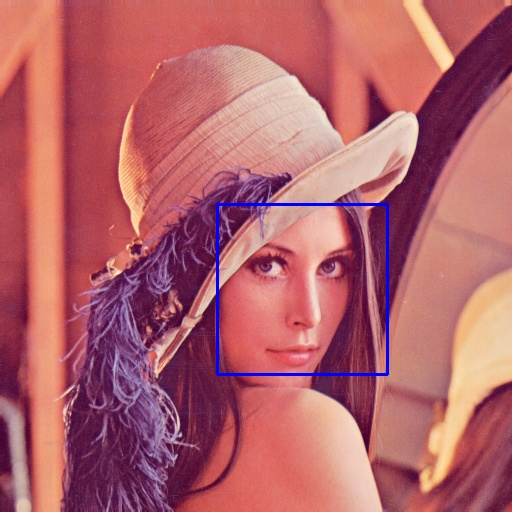
\includegraphics[width=\columnwidth]{result}
		% Create a subtitle for the figure.
		\caption{The Accuracy of training set and validation set}
		% Define the label of the figure. It's good to use 'fig:title', so you know that the label belongs to a figure.
		\label{fig:tf_plot}
		\end{center}
\end{figure}

\subsubsection{Face Detection:OpenCV}
Run the face\_detection.py file. Experience the OpenCV's built-in method of face detection using Haar Feature-based Cascade Classifiers.The result will be save as detect\_result.jpg ,as shown in Fig.2.

\begin{figure}[!hbt]
		% Center the figure.
		\begin{center}
		% Include the eps file, scale it such that it's width equals the column width. You can also put width=8cm for example...
		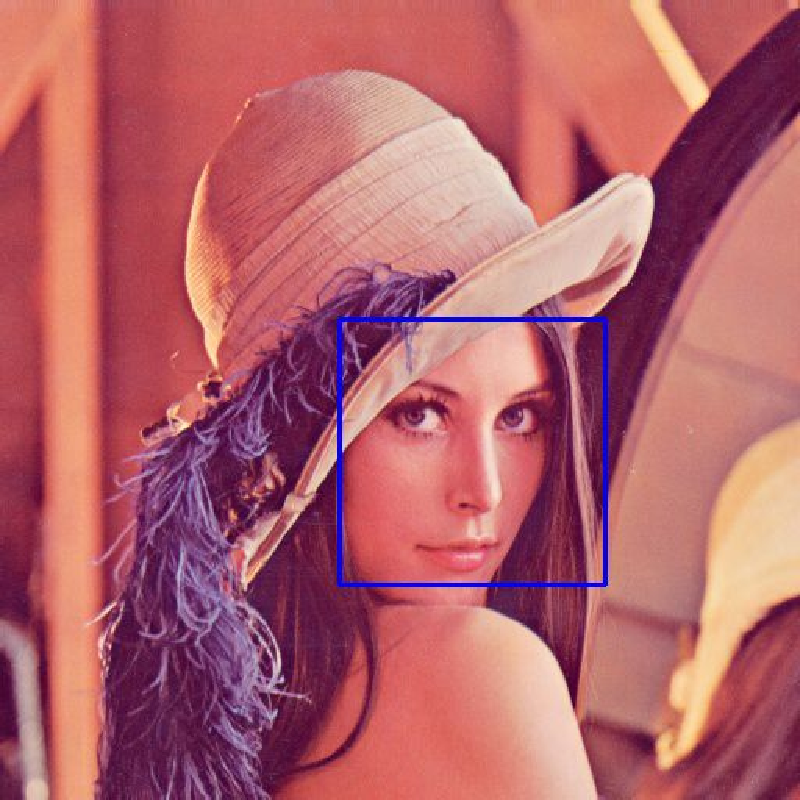
\includegraphics[width=\columnwidth]{luna}
		% Create a subtitle for the figure.
		\caption{The result of face\_detection.py}
		% Define the label of the figure. It's good to use 'fig:title', so you know that the label belongs to a figure.
		\label{fig:tf_plot}
		\end{center}
	\end{figure}
\section{Conclusion}
Through this experiment,I got a further understand of Adaboost Algorithm as well as experience the complete process of machine learning.The experiment result is also satisfied.
% Your document ends here!
\end{document}